\documentclass[10pt,a4paper]{article}

\usepackage[a4paper]{geometry}
\usepackage[utf8]{inputenc}
\usepackage{fancyhdr}
\usepackage{titlesec}
\usepackage{graphicx}

\title{\textbf{TP Algorithmique \& Programmation} \\ Coloriage d'images}
\author{Vincent Bonnecuelle et Jibril Saffi}
\date{Octobre 2015}

\pagestyle{fancy}
\fancyhead[R]{1AA}
\fancyhead[L]{Grenoble INP \-- Ensimag}

\renewcommand\thesubsection{\arabic{subsection}}

\titleformat{\subsubsection}
{\normalfont\large\bfseries}{Question \thesubsubsection}{1em}{}

\titleformat{\subsection}
{\normalfont\large\bfseries}{\thesubsection}{1em}{}

\titleformat{\section}[runin]
{\normalfont\large\bfseries}{}{1em}{}

\begin{document}
\maketitle
\hrule
\section*{Réponses aux questions}
\subsection{Lecture/écriture de données}
\subsubsection{} 
Nous avons identifié les cas d'erreurs suivants pour la fonction \texttt{pixmap::readMonochrome()}:
\begin{itemize}
\itemsep0em 
\item le fichier n'est pas du bon type;
\item il manque des valeurs dans le corps par rapport au header spécifié;
\item la forme du header n'est pas valide;
\item $n \cdot{m}$ ne renvoie pas un entier positif ou nul;
\item un commentaire est placé après le "nombre magique" P1.
\end{itemize}
Les tests unitaires correspondants à ces erreurs sont présents dans le fichier \textit{src/test/pixmap.cxx}.

\subsubsection{} 
Nous avons identifié les cas d'erreurs suivants pour la fonction \texttt{pixmap::writeColored()}:
\begin{itemize}
\itemsep0em 
\item le tableau bidimensionnel de pixels de couleur est vide;
\item le tableau bidimensionnel de pixels de couleur n'est pas rectangulaire (toutes les lignes doivent avoir la même longueur).
\end{itemize}
Les tests unitaires correspondants à ces erreurs sont présents dans le fichier \textit{src/test/pixmap.cxx}.

\subsubsection{}
L'implémentation de la fonction \texttt{randomMonochrome()} se trouve dans le fichier \textit{src/pixmap.cxx}.
\clearpage
\subsection{\texttt{MakeSet()} et \texttt{FindSet()}}

\subsubsection{}
Pour tester conjointement les fonctions {\texttt{MakeSet()} et \texttt{FindSet()} nous avons procédé à la création d'un ensemble avec {\texttt{MakeSet()} et la vérification de l'existence de ce dernier avec \texttt{FindSet()}.
Ce test est présent dans le fichier \textit{src/test/pixmap.cxx}.

\subsubsection{} \label{2.2}
La complexité de \texttt{MakeSet()} est égale à celle de \texttt{FindSet()} soit $O(1)$.
Concernant le co\^ut mémoire, \texttt{MakeSet()} est $O(n)$ tandis que \texttt{FindSet()} est $O(1)$.

\subsection{Union()}
\subsubsection{} \label{3.1}
Soit 2 ensembles disjoints $S_{1}$ et $S_{2}$ représentés par les listes chaînées $L_{1}$ et $L_{2}$. Afin de réaliser l'union de ces 2 ensembles, la solution naïve consiste à joindre la tête de $L_{2}$ à la queue de $L_{1}$ et de mettre à jour tous les éléments (dont le représentant) de $L_{2}$ afin que ces derniers pointent sur le représentant de $L_{1}$.

\begin{figure}[h]
\centering
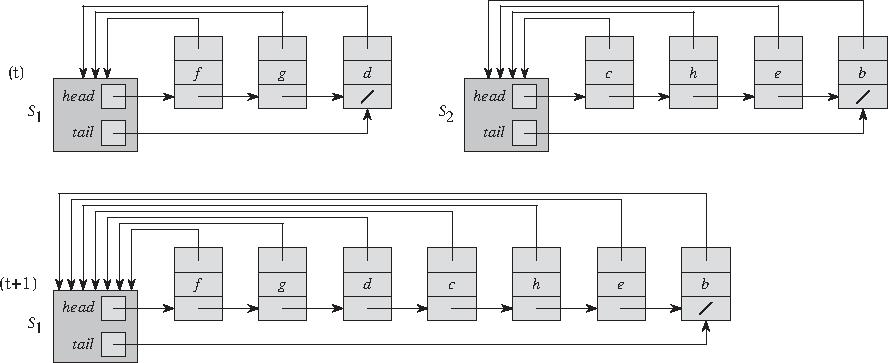
\includegraphics{3-1.pdf}
\caption{Mécanisme de \texttt{Union()}}
\end{figure}

Si l'on considère que le pire cas correspond au cas où chaque union ferait systématiquement parcourir l'ensemble le plus grand (pour mettre à jour les éléments). Alors pour $n$ unions on doit faire $n(n-1)?$ opérations\footnote{avec $k? = \sum\limits_{i=1}^{k}{i}$} d'où:
$$O(n(n-1)?) =  O(n(2(n-1))) = O(n^2)$$

Concernant le coût mémoire, aucunes variables supplémentaires n'est nécessaire car on se contente de modifier la structure d'une liste préalablement existante. Ainsi, le coût en mémoire serait de $O(1)$.
\subsubsection{}
La création d'un ensemble a pour complexité $O(1)$ donc $n$ créations d'ensembles aura pour complexité $O(n)$. Si l'on ajoute à cela $n$ unions successives, la complexité dans le pire cas atteint la valeur suivante :
$$O(n + (n-1)^2) = O(n^2)$$

\subsubsection{}
Dans la question~\ref{3.1} nous avons dégagé une problématique intéressante : si la taille de $L_{2}$ est supérieure à celle de $L_{1}$ nous sommes tout de même contraint de parcourir entièrement la liste $L_{2}$ pour pouvoir joindre celle-ci à $L_{1}$. Aussi, nous avons effectué une modification à la structure de données de liste chaînée : l'\textbf{ajout d'un champ représentant la taille de la liste}.

Grâce à cette information supplémentaire, il nous est désormais possible d'optimiser l'union de deux ensembles. Pour ce faire, on compare la taille des deux listes afin de systématiquement \textbf{joindre la tête de la liste la plus petite vers la queue de la liste la plus grande} et ainsi minimiser le temps de parcours nécessaire à la mise à jour des éléments.

\subsubsection{}
\textit{Voir fichier src/disjoint.hxx}

\subsubsection{}\label{3.5}
L'union implique nécessairement deux ensembles disjoints, nous réalisons donc au minimum $n-1$ opérations d'unions. Considérant un élément $x$ de la liste, nous savons que chaque fois que $x$ est mis à jour, il doit être contenu dans l'ensemble le plus petit. Aussi, la première fois que $x$ est mis à jour, l'ensemble résultant devra contenir au moins 2 éléments. De la même manière, la prochaine fois que $x$ est mis à jour, l'ensemble résultant devra quand à lui contenir au moins 4 éléments. En continuant ainsi, on remarque comme vu en figure~\ref{fig:tree}, que pour tout $k \leq n$, si $x$ a été mis à jour $\log(k)$ fois, l'ensemble résultant contient alors $k$ éléments.\\

\begin{figure}
\centering
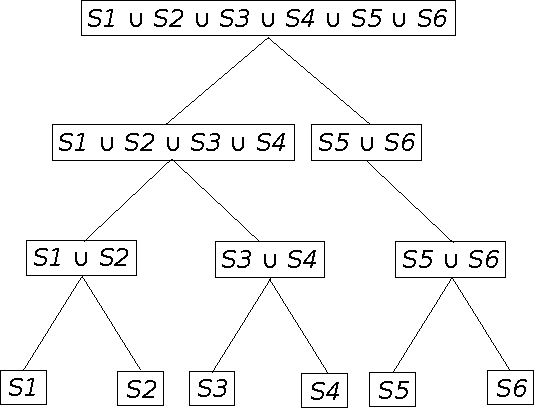
\includegraphics[scale=0.5]{3-5.pdf}
\caption{Les \texttt{Union()} décrivent un arbre binaire de profondeur $\log(n)$}
\label{fig:tree}
\end{figure}

Or l'ensemble le plus grand contient au maximum $n$ éléments, donc chacun de ces éléments est au moins mis à jour $\log(n)$ fois lors des opérations d'unions. Ainsi le temps total alloué à la mise à jour des éléments lors de toutes les opérations d'unions est : 
$$O(n\log(n))$$
De plus comme montré en~\ref{2.2} l'opération \texttt{MakeSet()} a une complexité $O(1)$ et on réalise $n$ opérations.
La complexité totale de la suite d'opérations est donc:
$$O(n+n\log(n)) = O(n\log(n))$$

\subsection{Algorithme général}
\subsubsection{}
Nous avons identifié les cas d'erreurs suivants pour la fonction \texttt{Disjoint::unite()}:
\begin{itemize}
\itemsep0em 
\item union d'un disjoint-set avec lui-même;
\item union d'un disjoint-set avec un ensemble vide.
\end{itemize}
Les tests unitaires correspondants à ces erreurs sont présents dans le fichier \textit{src/test/disjoint.cxx}.

\subsubsection{}
Soit $n$ et $m$ respectivement la longueur et largeur de l'image.
Comme vu en~\ref{2.2}, le coût en mémoire de \texttt{MakeSet()} est $O(1)$ et on réalise $n \cdot m$ créations d'ensembles, le coût total en mémoire est donc:
$$O(n\cdot{m})$$

Par ailleurs, d'après la réponse~\ref{3.5} pour $n\cdot{m}$ créations d'ensembles, la complexité asymptotique de l'algorithme est:
$$O((n\cdot{m})\log(n\cdot{m}))$$

\subsubsection{}

\subsection{Bonus}
Plut\^ot que d'ajouter la seconde liste à la fin de la première, on peut se contenter de l'insérer au début, l'ordre n'ayant pas d'importance.
Pour cela il nous faut tout de même accéder au dernier élément de la seconde liste, mais étant donné qu'on doit la parcourir pour mettre à jour ses pointeurs vers le représentant, on récupère ainsi simplement un pointeur vers celui-ci.

Il nous suffit ensuite de mettre à jour le dernier élément de la seconde liste et le pointeur vers la t\^ete de la première, exactement comme pour une \texttt{Union()} classique.
\vfill
\hrule
\begin{thebibliography}{9}
\bibitem{Introduction to algorithms} 
Charles E. Leiserson, Thomas H. Cormen, Clifford Stein and Ronald Rivest. 
\textit{Introduction to algorithms}. 
MIT Press, 1990.
\end{thebibliography}

\end{document}